\chapter{АНАЛИЗ ПРЕДМЕТНОЙ ОБЛАСТИ УПРАВЛЕНИЯ БЕСПИЛОТНЫМ АВТОМОБИЛЕМ}
В этой главе рассматривается обзор существующих систем управление беспилотными автомобилями.
Определены основные принципы и выделены основные подсистемы системы управления. Произведен
обзор способов построения траекторий движения и способов удержания этой траектории.

\section{Обзор применяемого аппаратного обеспечения}

Беспилотные автомобили должны функционировать в условиях сложной окружающей среды с большим
количеством различных неподвижных и движущихся препятствий различных конфигураций, в окружении
других участников дорожного движения, пешеходов и т.п. Для обеспечения высокого уровня
безопасности для пассажиров и других представителей дорожного движения беспилотный автомобиль
должен оперативно и адекватно реагировать на изменяющиеся условия окружения, для этого автомобиль
должен быть оснащен различными датчиками и реализовывать надежные и эффективные алгоритмы обработки данных.

Важным этапом в развитии беспилотных автомобилей были соревнования Darpa Grand Chellenge (2004г, 2005г)
и Darpa Urban Challenge (2007г), в ходе которых команды соревновались в разработке и постройке
беспилотного автомобиля, который сможет самостоятельно проехать в трассу в загородных условиях
(2004г, 2005г) и в городских условиях (2007г). Некоторые команды опубликовали ряд работ, в
которых описаны подходы, использованные ими при разработке беспилотного автомобиля.

Главным датчиком большинства беспилотных автомобилей ялвяется 3D LIDAR (Light Identification Detection and
Ranging) ~--- вращающийся многолучевой лазерный дальномер, позволяющий получать данные о конфигурации окружающего
пространства в трехмерном пространстве на большом расстоянии. Так, например, ЛИДАР Velodyne HDL-64E способен
обнаруживать объекты с высокой отражающей способностью (например, автомобили) на расстоянии до 120 м, а объекты
с низкой отражающей способностью на расстоянии до 50 метров \cite{sensor_hdl64_manual}.  ЛИДАР позволяет получить большое
количество информации об окружающем пространстве и с его помощью значительно легче и надежнее реализовать такие задачи,
как обнаружение препятствий, определение дороги и т.п.  Из рассмотренных команд, участвовавших в Darpa Urban Challenge:
Junior (Стэнфордский университет) \cite{darpa_junior}, Talos (Массачусетский технологический институт)\cite{darpa_mit},
BOSS (несколько участников из университета Карнеги-Меллона, компаний General Motors,  Caterpillar, Continental, Intel)
\cite{darpa_boss}, AnnieWAY (технологический институт Карлсруэ) \cite{darpa_annieway} все команды использовали
шестидесятилучевой лучевой ЛИДАР Velodyne HDL-64E в качестве основного источника информации об окружающем пространстве.
Дополнительно применялись однолучевые 2D-ЛИДАРЫ в различных конфигурациях, для того, чтобы получить лучшее
покрытие слепых зон, расположенные по бокам, на переднем и/или заднем бамперах, на крыше. ЛИДАРы не лишены
недостатков. Главным их недостатком является высокая стоимость, что делает их не лучшим кандидатом для применения
в массовых коммерческих автомобилях, так например шестнадцатилучевой ЛИДАР Velodyne VLP-16 стоит дороже ряда
бюджетных автомобилей. Помимо этого, работа ЛИДАРа затруднена или вовсе невозможна в  дождь, снег,
туман.

Несмотря на большой объем и сравнительно высокую точность данных, получаемых с помощью ЛИДАРа, одного ЛИДАРа не
достаточно для построения системы компьютерного зрения беспилотного автомобиля. В дополнение к ЛИДАРам, все
системы комплектуются одной, но чаще несколькими, цветными и/или черно-белыми камерами, а также радарами.

Камеры, наряду с ЛИДАРом, являются важнейшими датчиками системы компьютерного зрения беспилотного автомобиля.
С помощью камер производится распознавание дорожных знаков, светофоров, дорожной разметки. В настоящее время,
в связи со значительным прогрессом в области искусственных нейронных сетей, можно с высокой точностью производить
детектирование различных объектов \cite{cv_nn_object2d_review}, как в 2D \cite{cv_nn_object2d_ssd2}, так и в 3D
\cite{cv_nn_object3d_voxelnet2}, \cite{cv_nn_object3d_pointnet2}, а также
сегментацию \cite{cv_nn_segmentation_deeplabv3}, т.е. определять, какие пиксели изображения относятся к тем и или иным к классам, таким образом
можно детектировать дорогу и ровное пространство, доступное для движения. Прогресс в этой области делает возможным реализацию системы компьютерного
зрения для беспилотного автомобиля без использования ЛИДАРа, что существенно снижает сложность и стоимость такой
системы, что важно для серийных автомобилей. В настоящее время автомобили Tesla, оснащенные автопилотом
с ограниченной функциональностью, используют только камеры. Тем мне менее, использование ЛИДАРа
значительно увеличивает точность и надежность системы, и ЛИДАРы используются во всех проектах
беспилотных автомобилей. Комбинируя данные с ЛИДАРа и камер (так называемая задача sensor fusion), можно
существенно повысить точность таких задач, как распознавание и отслеживание препятствий, определение дороги.

Другим важным датчиком, применяемым в беспилотных автомобилях, является радар. За последние годы применение радаров
в автотранспорте (automotive radar) активно развивалось. Применение радов не ограничивается полностью беспилотными
автомобилями, они находят место и в обычных автомобилях в системах помощи водителю (advanced driver-assistance
system, ADAS) и в системах активной безопасности \cite{sensor_radar_overview}, \cite{sensor_radar_overview_2}.
Радары обладают рядом возможностей, недоступных другим датчикам, таких как возможность работы вне зависимости от
погодных условий и уровня освещенности, большая (до 200м) дальность, возможность определять положение
объектов и непосредственно определять их скорость с помощью эффекта Доплера.

Например, команда BOSS \cite{darpa_boss} в Darpa Urban Challenge применяла радар совместно с ЛИДАРом для отслеживания
объектов. Объекты отслеживались независимо, используя особенности датчиков (непосредственное измерение скорости объектов
с помощью радара играло важную роль в алгоритме отслеживания) и затем результаты объединялись.

В таблице \ref{tab:sensors_compare} приведено сравнение основных свойств и областей применения рассмотренных
выше датчиков.

\begin{table}[h]
    \caption{Сравнение применяемых датчиков}
    \label{tab:sensors_compare}
    \begin{tabularx}{\textwidth}{|X|X|X|X|X|}
        \hline
        Датчик        & Получаемая информации & Дальность & Влияние освещенности & Влияние погодных условий  \\
        \hline
        Камера        & Цветное или ч/б изображение & Не позволяет определить расстояние  & Да & Да \\
        \hline
        Стереокамера  & Облако точек & до 20 м & Да & Да \\
        \hline
        3D ЛИДАР      & Облако точек $360\degsym$  & до 120 м  & Малое & Да \\
        \hline
        2D ЛИДАР      & Положение препятствий (2D) & до 20 м \cite{jetson_car_zed} & Малое & Да \\
        \hline
        Радар         & Положение и скорость препятствий (2D) & до 200 м & Нет & Нет \\
        \hline
    \end{tabularx}
\end{table}

\section{Обзор общей структуры системы управления беспилотными автомобилями}

Несмотря на то, что было представлено большое количество различных систем управления беспилотными
автомобилями, все они обладают схожей структурой. В общем виде, систему управления беспилотным автомобилем
можно разделить на следующие подсистемы:
\begin{itemize}
    \item интерфейс сенсоров, позволяющий получать данные от сенсоров;
    \item подсистема восприятия (perception), осуществляющая построение комплексной информации об
          окружающем пространстве, на основе данных от сенсоров, определяя положение автомобиля,
          дорогу, статические и динамические препятствия, распознавания дорожные знаки, светофоры, разметку,
          и формирующая в конечном итоге цифровую карту окружающего пространства, которая в дальнейшем
          используются другими подсистемами;
    \item подсистема управления движением,осуществляющая принятие решений и построение безопасной
          и достижимой траектории и осуществляющая движение по траектории, формирования управляющих сигналов,
          таких как угол поворота руля, газ, тормоз.
\end{itemize}

Подобная высокоуровневая архитектура применена как командами Darpa Urban Challenge \cite{darpa_junior}, \cite{darpa_mit},
\cite{darpa_boss}, \cite{darpa_annieway}, так и описана в более современных статьях,
таких как \cite{developing_car_1}, \cite{car_proud}, \cite{car_race}.

Архитектура обобщенной системы управления автономным автомобилем, построенная на основе анализа ряда
работ \cite{motion_planning_review}, представлена на рисунке \ref{img:general_arch}.

\begin{figure}[h]
    \centering
    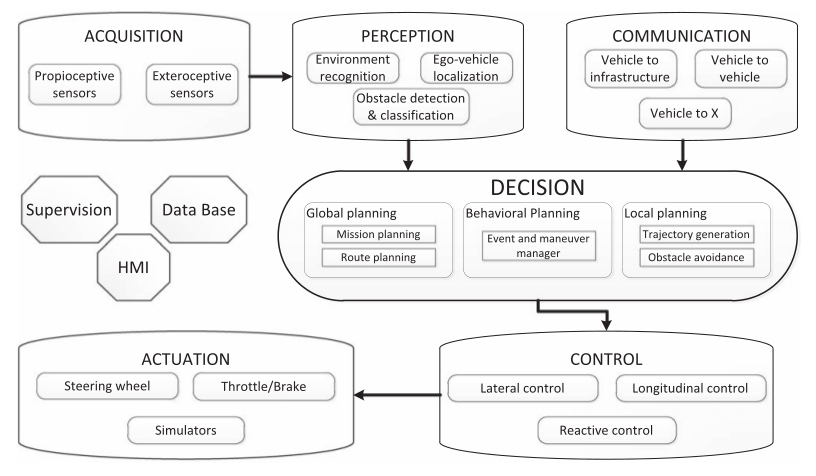
\includegraphics[width=\linewidth]{images/general_arch}
    \caption{Обобщенная абстракция архитектуры управления автономными автомобилями \cite{motion_planning_review}}
    \label{img:general_arch}
\end{figure}

Подсистема восприятия обычно состоит из следующих компонентов, состав и взаимодействие которых, в прочем, могут
отличаться в зависимости от назначения и уровня автономности беспилотного автомобиля:
\begin{itemize}
    \item подсистема локализации, осуществляющая определения положения автомобиля с помощью GPS и системы одновременной
          картографии и навигации (SLAM),
    \item подсистема выделения дороги (ground detection/road detection), определяющая, какие области пространства вокруг
          доступны для передвижения,
    \item подсистема детектирования (object detection)  и отслеживания (object tracking) объектов, позволяющая определять
          положение динамических препятствий вокруг автомобиля и их скорость и направление движения,
    \item подсистемы распознавания дорожных знаков, светофоров, дорожной разметки и т.п.
\end{itemize}

Процесс планирования движения и принятия решений в современных беспилотных автомобилях обычно представлен в виде
иерархии: планирование маршрута (route planning), принятие решений (behaviour planning, decision making), локально
планирование (local motion planning) и управление с обратной связью \cite{motion_planning_review_2}. Точное разделение на
уровни обычно размыто и может отличаться в различных работах, но общая структура сохраняется. Пример того, как
разделяются задачи по уровням иерархии представлен на рисунке  \ref{img:planning_hierarchy}.

\begin{figure}
    \centering
    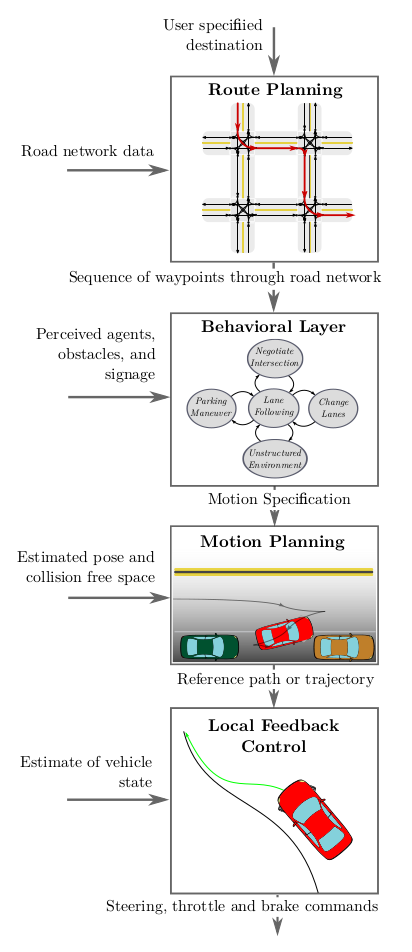
\includegraphics[height=\textheight-3cm]{images/planning_hierarchy} % ха-ха, костыль
    \caption{Иерархия системы управления}
    \label{img:planning_hierarchy}
\end{figure}

На верхнем уровне осуществляется планирование маршрута по дорожной сети. Затем следуют уровень планирования поведения,
который принимает решения и формирует локальные навигационные задачи, которые приближают автомобиль к выполнению
высокоуровневой задачи и удовлетворяют правилам дорожного движения. Затем локальный планировщик формирует непрерывный
путь в окружающем пространстве, который выполняет локальную навигационную задачу. Система управления с обратной связью
осуществляет выполнение запланированного
движения и коррекцию ошибок.

Система планирования маршрута должна выбирать как можно более оптимальный путь по дорожной сети от текущего
положения к точке назначения. Типичным решением является представление дорожной сети как ориентированного
графа, ребрам которого назначаются веса, соответствующие стоимости движения по данному сегменту дороги
(в простейшем случае ~--- расстояние). Тогда задача построения маршрутка может быть сформулирована как задача
нахождения пути на графе с наименьшей стоимостью. Участники Darpa Urban Challenge решали эту задачу самостоятельно,
использую хорошо известные алгоритмы, такие как алгоритмы Дейкстры, А* или их модификации. Это было возможно, потому что
область проведения Darpa Urban Challenge была небольшая. В реальных сценариях применение простейших алгоритмов
невозможно, потому что дорожная сеть может содержать миллионы узлов. Но это и не требуется, потому что в настоящее
время в настоящее время существует большое количество картографических сервисов, реализующих эффективные алгоритмы
построения маршрутов вплоть до континентального масштаба и  предоставляющих подобную функциональность в виде API.
Поэтому в данной работе не рассматривается глобальное планирование маршрута, так как реализовывать его самостоятельно
не имеет смысла.

После того, как глобальный маршрут был построен, автономный автомобиль должен уметь двигаться по этому маршруту и
взаимодействовать с другими участниками дорожного движения в соответствии с правилами дорожного движения. Планировщик
поведения отвечает за выбор подходящего поведения в каждый момент времени, основываясь на наблюдаемой дорожной
ситуации. Например, когда автомобиль достигает стоп-линии, планировщик поведения формирует команду остановки.
Правила дорожного движения определяют правильно поведения в различных ситуациях. Варианты поведения и возможные
дорожные ситуации представляют собой конечные множества, поэтому естественным будет представление планировщика
движения в виде конечного автомата. Большинство участников DARPA Urban Challenge применяли конечные автоматы для
задачи принятия решений.

Основной проблемой является неопределенность намерений остальные участников дорожного движения. Проблема предсказания
намерений участников движения активно изучается и существуют различные подходы, от простой линейно экстраполяции
\cite{darpa_junior_frenet} движения до предсказания движения с помощью Deep Learning \cite{nn_motion_prediction},
что является наиболее перспективным способом в настоящее время. Неопределенность поведения участников дорожного движения
часто учитывается в планировании поведения спомощью вероятностного формализма, например, применяя марковский процесс
принятия решений.

После того, как планировщик поведения определил поведение, которое должно выполняться в данной дорожной ситуации,
например, удерживать полосу, выполнит обгон или остановиться на светофоре, выбранное поведение должно быть
представлено в виде пути или траектории, которые, в свою очередь, могут быть выполнены низкоуровневым регулятором с
обратной связью. Эта траектория должна избегать препятствий, быть достижимой для автомобиля согласно его кинематике
и динамике и, наконец, быть комфортной для пассажиров. Эта задача соответствует стандартной задаче планирования
движения (motion planning) в робототехнике.

И, наконец, регулятор с обратной связью отвечает за то, чтобы сформировать управляющие сигналы, такие как поворот
руля, газ и торможение, чтобы точно следовать программной траектории.

\section{Обзор методов планирования движения}

Локальный планировщик движения отвечает за формирование безопасной, достижимой и комфортной для пассажиров траектории
из текущего положение автомобиля до следующей цели, определенной планировщиком поведения. В зависимости от ситуации,
это могут быть различные цели, такие как удержание полосы, следование на заданном расстоянии от впереди идущего
автомобиля, остановка и др. Планировщик движения учитывает информацию о статических и динамических препятствиях, чтобы
сгенерировать траекторию, которая будет избегать препятствий и будет выполнима с точки зрения кинематики и/или динамики
автомобиля. В некоторых подходах рассматривается формирование оптимальной по отношению к некой целевой функции
траектории.

Получаемое программное движение может представлено в виде пути или траектории. В случае планирования пути, результатом
будет путь в конфигурационном пространстве автомобиля,

Задача планирования движения (motion planning) в робототехнике ~--- процесс разбиения требуемого движения
на дискретные действия, которые удовлетворяют ограничениям. Планирование движения является важной задачей
робототехники и активно  исследуется и разрабатывается в течении последних десятилетий. Разработано большое
количество алгоритмов планирования движения, как для решения задачи в общем случае, так и для конкретных
приложений. В этом разделе дается обзор методов, позволяющих осуществить задачу локального планирования
беспилотного движения автономного автомобиля.

Существует большое количество методов, позволяющих решить данную задачу, такие как методы поиска на графах,
случайные методы поиска (sample-based motion planning), методы интерполяции движения кривыми, методы
численной оптимизации и другие. Обзор методов планирования движения в приложении к беспилотным автомобилям
рассмотрен в работах \cite{motion_planning_review},
\cite{motion_planning_overview_obstacles}, \cite{motion_planning_overview_modern},
\cite{motion_planning_review_2}, \cite{motion_planning_review_3}.

Различные способы планирования движения имеют свои преимущества и недостатки. Например, одни методы позволяют
более поло решать задачу планирования движения, но являются более вычислительно сложными, что затрудняет их
применение в реальном времени на дорогах с быстро меняющейся ситуацией.  Чтобы решить эту проблему, многие
команды в DARPA Urban Challenge не ограничивались одним способом планирования движения. Распространенным подходом
было применять один планировщик движения при движении по дорогам, а другой - при движении в неструктурированном окружении,
например, при задаче парковки.

Задача планирования движения в применении к автомобилю в общем виде является нетривиальной, потому что
динамика автомобиля описывается сложными дифференциальными уравнениями, имеющими, что немаловажно,
неголономные связи \cite{car_frund}\hl{правильно написать}. Многие исследователи применяют различные упрощенные модели динамики
автомобиля \cite{car_dynamics_1}. Очень распространенной является "велосипедная" модель динамики
автомобиля, которая применяется в ряде работ \cite{car_dynamics_bycicle_model_1}, \cite{car_dynamics_bycicle_model_2},
\cite{darpa_annieway_navigation}.


\subsection{Формулирование задачи планирования движения}
Перед рассмотрением алгоритмов планирования движения необходимо определить несколько понятий, которые
применяются в теории автоматизированного управления и сформулировать задачу планирования движения.

Конфигурационное пространство $\CST$ системы ~--- это совокупность всех ее обобщенных координат.

Дано:
\begin{itemize}
    \item пространство конфигураций $\CST$ робота;
    \item множество конфигураций, соответствующее препятствиям $\CST_o \in \CST$, соответственно
          множество свободных конфигураций $\CST_{free} = C \setminus C_o$;
    \item начальные и конечные конфигурации $q_s$, $q_g$.
\end{itemize}

Задача планирования движения может быть сформулирована как планирование пути или планирование траектории.
В первом случае, требуется найти функцию $\tau(\alpha): [0,1] \rightarrow \CST_{free}$, представляющую путь робота в
конфигурационном пространстве, где $\tau(0)=q_s$, $\tau(1)=q_g$. В этом случае, решение не определяет, как этот пройден
автомобилем. Планировщик движения может выбрать профиль скорости для этого пути, как это сделано в \cite{darpa_boss},
или делегировать эту задачу нижележащим подсистемам.

В случае планирования траектории, явно учитывается время движение. В таком случае требуется найти функцию
$\pi(t) : [0, T] \rightarrow C$, где $T$ - горизонт планирования. В отличие от планирования пути, планирование
траектории явно указывает, как должна меняться конфигурация с течением времени.

\hl{Требуется это более внятно и корректно сформулировать}.

\subsection{Методы поиска на графах}
Для решения задачи планирования движения можно применять алгоритмы поиска на графах, такие как
алгоритм Дейкстры, алгоритм A* или их модификации. Для применения алгоритмов поиска на графах к задаче
планирования движения необходимо сначала представить конфигурационное пространство в виде графа.

В данном методе большую роль играет способ построения графа, а именно выбор опорных точек и ребер,
которые их соединяют.

Простейшими, но крайне широко распространенными вариантами представления конфигурационного пространства
в виде графа являются методы клеточной декомпозиции. Наиболее распространенным вариантом является приближенная клеточная
декомпозиция, когда пространство разбивается с помощью равномерной сетки (grid map)
\cite{motion_planning_overview_obstacles}. Преимуществом этого метода является то, что его легко реализовать и легко
представить конфигурацию окружающего пространства в виде сетки. Этот метод широко применяется в ряде существующих
реализаций поиска пути, таких как navigation stack в ROS \cite{ros_navigation}. Недостатком этого метода является существенное
увеличение размера графа при уменьшении шага дискретизации, увеличении области, в которой осуществляется планирование и,
особенно, при увеличении размерности  конфигурационного пространства. Подобные методы в основном применяются для
геометрического планирования на плоскости, с увеличением числа степеней свободы (повороты, трехмерное пространство,
трехмерное пространство с поворотами) количество вершин в графе становится слишком большим для эффективного применения
данного метода.

Другим способом выбора опорных точек графа является использование диаграммы видимости.
\cite{motion_planning_overview_obstacles} Диаграмма видимости определяется как неориентированный граф, вершины которого
включают множество вершин препятствий, а ребра соединяют некоторые вершины таким образом, что никакое ребро не
пересекается с препятствиями. Для использования диаграммы видимости необходимо, чтобы препятствия имели форму
многоугольника или многогранника. Поскольку путь строится по вершинам препятствий, и часть пути совпадает с краями
препятствий, существует определенная опасность столкновения с препятствиями. Кроме того, при увеличении количества
препятствий возрастает сложность графа, причем этот рост очень быстрый. Подобный подход редко применяется для
беспилотных автомобилей.

Еще одним методом построение графа, который сильно распространен в задачах планирования \cite{darpa_annieway_navigation},
\cite{motion_planning_overview_obstacles}, являются диаграммы Вороного. Диаграмма Вороного конечного множества точек на
плоскости представляет собой разбиение плоскости таким образом, что каждая область образует геометрическое место точек
(локус), каждая из которых более близка к одному элементу множества, чем к другому. Преимуществом диаграмм Вороного для
планирования движения является то, что с их помощью можно построить путь, наиболее удаленный от всех препятствий, и,
следовательно, наиболее безопасный.

Команда "BOSS" Darpa Urban Challenge применяла метод поиска на графах для планирования движения \cite{darpa_boss},
\cite{darpa_boss_2}, \cite{darpa_boss_3}. Для графа они применяют т.н. решетку состояний (state lattice). Узлы
графа представляют собой дискретизированные состояния в пространстве конфигураций, а каждое ребро графа представляет
достижимый путь. В отличие от более распространенных подходов, применяющих сетки, клетки которых просто имеют 4
или 8 соединенных соседей, в этом подходе гарантируется, что полученный путь будет достижимым.

Наиболее применительны методы поиска на графах для планирования движения в неструктурированном окружении.

Далее будут рассмотрены некоторые модиификации известных алгоритмов поиска пути на графах, ориентированные на
нахождение кинематически и динамиески достижимых путей.

\subsection{Hybryd A*}
Из-за нелинейной динамики автомобиля, путь, построенный с помощью поиска на
регулярной прямоугольной дискретной сетке будет кинематически и динамически недостижим для автомобиля.
Было предложено много вариантов решения этой проблемы, так например, алгоритм Hybrid A*
\cite{motion_planning_hybrid_a_star}, предложенный командой "Junior" DUC \cite{darpa_junior}.
В отличие от алгоритма A*, примененного к регулярной сетке, имеющий 4 или 8 дискретных соединений между соседними
ячейками, Hybrid A* формирует набор траекторий, учитывающих нелинейную динамику и непрерывную природу движения
автомобиля (рисунок \ref{img:hybrid_a_star}).

\begin{figure}[h]
    \centering
    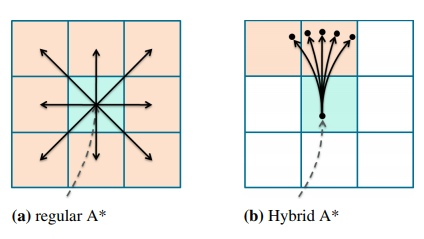
\includegraphics[]{images/hybrid_a_star}
    \caption{Hybrid A* в сравнении с A* \cite{darpa_junior}}
    \label{img:hybrid_a_star}
\end{figure}

Алгоритм работает с дисркетными сетками в трехмерном пространстве состояний $x, y, \theta$, где $x, y$ - положение
автомобиля, а $theta$ - ориантация. Рассмотрим работу алгоритма. Допустим, что в некий момент времени состояние
автомобиля $<x, y, \theta>$ и оно соответствует ячейке $c_i$ в дискретизированном пространстве состояний. Сопоставим
с этой ячейкой непрерывные координаты: $x_i = x$, $y_i = y$, $\theta_i = \theta$. Далее решаем задачу прямой дианмики,
интегрируя движение автомобиля при подаче управления $u$ в течении заданного времени $t$. Конечным состоянием будет
$<x', y', \theta'>$, попадаяющее в дискретную клетку $c_j$. Аналогичным образом сопоставим непрерывные координаты с
этой клеткой: $x_j = x'$, $y_j = y'$, $\theta_j = \theta'$. Это позволяет гарантировать, что мы имеем непрерывную
траекторию из клетки $c_i$ и $c_j$, для которой гарантируется кинаматическая и динамическая достижимость
(разумеется, при использовнии достаточно точной динамической модели), а также соответствующее управление $u$,
что не гарантируется для обычного A* алгоритма. Дальнейший поиск по этому графу осуществляется аналогично обычному
алгоритму A*.


\subsection{State Lattice}
Другой широко распространенной модификацией графовых алгоритмов является семейство алгритмов, называемых в англоязычной
литературе "State Lattice" (решетка состояний). Алгоритм был предложен в работе \cite{motion_planning_lattice_1} и
близок по своей идее к алгоритму Hybrid A*, рассмотренному ранее. В работе представлено пространство поиска,
называемое решеткой состояний, позволяющее представить планирование неголономного движения как задачу поиска на графе.

Решетка состояний представляет собой дискретное множество всех достижимых конфигураций системы. Ее построение
осуществляется путем дискретизирования пространства состояний в виде многомерной решетки, состоящих
из достижимых состояний, и попытки соединить начальное состояние со всеми узлами решетки с помощью достижимых путей
в качестве ребер. В общем случае, решетка состояний содержит все достижимые пути (с заданной дискретизацией), что
подразумевает, что если автомобиль можете переместиться из одного состояния в другое, то решетка состояний содержит
последовательность путей для осуществления этого маневра.

Подобно обычной сетке, решетка состояний преобразует задачу планирования в непрерывном пространстве в задачу формирования
последовательности выбора из нескольких дискретных альтернативных состояний, но в отличие от обычной сетки, решетка
состояний строится таким образом, что ее связи являются достижимыми путями.

Построение решетки состояний требует решение обратной задачи для нахождения достижимого пути между двумя заданными
состояними. Существует ряд методов, позволяющих решить эту задачу. Несмотря на то, что метод решетки состояний по-прежнему
требует решения обратной задачи, что, как было замечено выше, является нетривиальной задачей, этот метод существенно
упрощает задачу планирования движения, потому что позволяет осуществлять планирование движения в виде графа в условиях
наличия различных препятствий, позволяя формировать сложную траекторию, что существенно более затруднено при применении
чисто математических методов решения этой задачи. В данном случе требуется решать обратную задачу лишь для некого ограниченного
множества возможных комбинаций начальных и конечных состояний.

Друим немаловажным свойством этого метода является то, что в силу использования регулярной сетки, можно выделить набор
состояний, инвариантный к пространственному перемещению (рисунок \ref{img:lattice_overview}). Это позволяет заранее
расчитать ограниченный набор состояний и соответствующих траекторий и управлений с помощью точных моделей и
ресурсозатратных алгоритмов, а в процессе планирования движения в реальном времени позьоваться этой заранее расчитанной
таблицей. Этот подход широко применяется в ряде разработок, например, в автомобиле "BOSS" DUC \cite{darpa_boss}.

\begin{figure}[h]
    \centering
    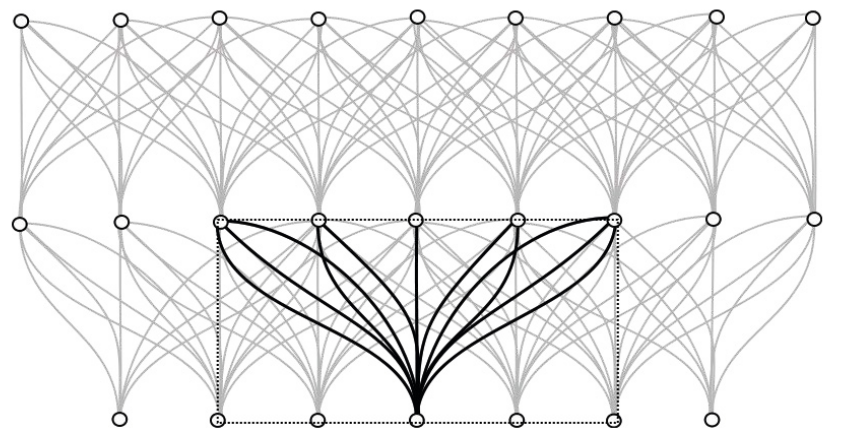
\includegraphics[]{images/lattice}
    \caption{Пример регулярной решетки состояний.  Базовое множество управлений и результирующих
             путей (черный) не зависит расположения и может быть продублирован. Это позволяет
             очень эффективно представлять множество траекторий и решать проблему планирования
             движения \cite{motion_planning_lattice_2}}
    \label{img:lattice_overview}
\end{figure}

Важным понятияем в этом методе является понятие эквивалентности путей. Путь $\tau_1$ считается эквивалентным пути
$\tau_2$, если $\tau_1$ содержится в определенном регионе $Q$ вокруг $\tau_2$ (рисунок \ref{img:lattice_path_eq}).
Все пути, являющиеся эквивалентными, представляются одним путем.

Для достижения эффективности, как было сказано выше, возможно дублирование некого базового набора состояний и траекторий
для разных начальных состояний, таким образом позволяя возможность эффективно конструировать граф необходимого размера
в реальном времени. Для реализации такой возможности во всем множестве путей, которое представляет сосбой решетка состояний,
необходимо выделить базовое множество. Например, ддя обычной регулярной сетки, каждая ячейка которой соединена с
четырьмя соседними, базовым множеством путей будет движение на одну клетку вперед, назад, влево и вправо. Этого простого
набор путей достаточно, чтобы описать любые перемещения в этом пространстве состояний. Для решетки состояний применяется
подобная идея. Любой путь через решетку может быть декомпозирован в последовательность путей из некого минимального
набора таким образом, что эта последовательность будет эквивалентной исходному пути.

\begin{figure}[h]
    \centering
    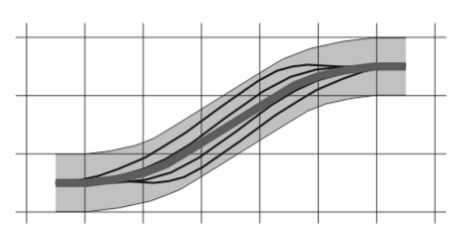
\includegraphics[]{images/lattice_path_eq}
    \caption{Эквивалентность путей. Множество различных путей (черные линии), которые содержаться в пределах заданного
             региона (серая область), считаются эквивалентными}
    \label{img:lattice_path_eq}
\end{figure}

\subsection{Случайные методы}

При решении задач планирования движения в пространствах высоких размерностей, которые часто возникают в современной
робототехнике (например, планирование движение твердого тела в трехмерном пространстве с шестью степенями свободы или
планирование движения многозвенного манипулятора), классические методы, такие как методы поиска на графах, обладают
очень большой вычислительной сложностью. Для решения таких задач перспективными являются случайные (sample-based) методы,
такие как Probabilistic roadmap, Rapidly-exploring random graph (RRG), Rapidly-exploring random tree (RRT)
\cite{motion_planning_rrt}, Optimal Rapidly-exploring random tree (RRT*)\cite{motion_planning_rrt_star}.

Идея метода заключается в том, что начиная из начального состояния строится дерево, которое может достичь конечного
состояния, путем выбора случайных точек в конфигурационном пространстве. Алгоритм RRT представлен в листинге
\ref{alg:rrt}, а иллюстрация метода $EXTEND$ на рисунке \ref{img:rrt_extend}.

\begin{algorithm}
    \caption{ Rapidly-exploring random tree }
    \label{alg:rrt}
    \begin{algorithmic}
        \Function{RRT}{$x_{init}$}

            $\tau.init(x_{init})$
            \For{ $k=1$ to $K$ }
                \State $x_{rand} \leftarrow RANDOM\_STATE()$
                \State EXTEND($\tau$, $x_{rand}$)
            \EndFor
        \EndFunction
        \Function{EXTEND}{$\tau$, $x$}

            $x_{near} \leftarrow NEAREST\_NEIGHBOUR(x, \tau)$
            \If{$NOT\_COLLIDED(x, x_{near}, x_{new})$}
                \State $\tau.add\_vertex(x_{new})$
                \State $\tau.add\_edge(x_{near}, x_{new}, u_{new})$
                \If {$x_{new} = x$}
                    \State \Return REACHED
                \Else
                    \State \Return ADVANCED
                \EndIf
            \EndIf
            \Return TRAPPED
        \EndFunction
    \end{algorithmic}
\end{algorithm}

\begin{figure}[h]
    \centering
    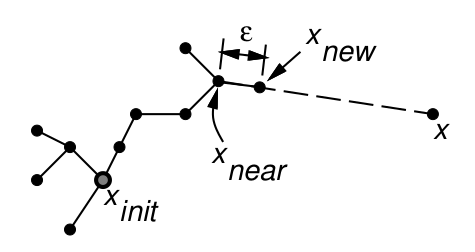
\includegraphics[]{images/rrt_extend}
    \caption{Пример работы метода EXTEND алгоритма RRT}
    \label{img:rrt_extend}
\end{figure}

Особенность этого семейства алгоритмов, как и многих других итерационных методов, является их сходимость
в пределе, т.е. решение будет получено при количестве
итераций стремящемся к бесконечности. Тем не менее, практическое использование этого семейства алгоритмов
позволяет быстро находить решение для высоких размерностей. Это свойство является преимуществом для систем
реального времени, которым является беспилотный автомобиль. Для систем реального времени ключевой является
способность выполнять работу в строго определенный интервал времени. К примеру, под планирование локальной
траектории вперед на заданный горизонт планирования отводится 0.5 секунды, и превышение этого времени может
привести к нарушению функционирования беспилотного автомобиля, что может создать опасную ситуацию.  В случае
с RRT алгоритмами, указывается максимальное время работы, после которого итерационный процесс прекращается.
В этом случае, полное решение может быть не найдено, но планирование может быть повторено через некоторое
время, чтобы построить недостающий участок пути.

Для применения этого алгоритма достаточно определить процедуру проверки на пересечение с препятствием
$NOT\_COLLIDED$.

Существует большое количество модификаций алгоритма RRT, особенно необходимо отметить алгоритм RRT*
\cite{motion_planning_rrt_star}, являющийся асимптотически-оптимальной версией алгоритма RRT. Он основан на
на алгоритме rapidly-exploring random graph (RRG) и имеет отличающуюся процедуру добавления новой точки в граф.
В отличие от алгоритма RRT, который прекращает свою работу, когда решение было найдено, алгоритм RRT* продолжает
работу, постепенно находя все более оптимальные решения.

Отдельно стоит выделить направление под названием кинодинамическое планирование (kinodynamic planning), которое
является актуальным в последнее время. В этом случае планирование осуществляется не в конфигурационном пространстве,
а в пространстве состояний (фазовом пространстве) \cite{motion_planning_kinodynamic_rrt}, которое определяется
следующим образом. Пусть $\CST$ ~--- конфигурационное пространство, каждая конфигурация $q \in \CST$ представляет
положение робота в пространстве. Обозначим пространство состояний как $\XST$, в котором состояние $x \in \XST$
определяется как $x = (q, \dot{q})$. (Состояние может определяться и с использованием производных высших порядков).

Это позволяет осуществлять планирование не только с учетом кинематической модели автомобиля, но и с учетом
динамической модули с дифференциальными ограничениями и неголономными связями.
Таким образом, результирующие пути будут достижимы с точки зрения динамики автомобиля, что
не всегда возможно для других методов планирования, что приводит к необходимости вводить различные искусственные
ограничения. Результатом такого метода планирования может быть не только траектория в пространстве
состояний, которая подается на вход низкоуровневого регулятора с обратной связью, но и непосредственно
последовательность управляющих сигналов, которые приведут систему к движению с такой траекторией.

Для реализации этих алгоритмов необходимо определить функции $PROPAGATE$ и $STEER$. Функция $PROPAGATE$
(\ref{eq:rrt_propagate}) формирует следующее состояние системы после применения к ней заданного управляющего
воздействия, например, путем численного интегрирования.
\begin{equation}
    \label{eq:rrt_propagate}
    x_{i+1} = PROPAGATE(x_i, u_i, \Delta t)
\end{equation}

\noindent\begin{tabularx}{\linewidth}{lllX}
    где & $x_i$      &~---& текущее состояние, \\
        & $u_i$      &~---& управление, \\
        & $\Delta t$ &~---& время интегрирования.
\end{tabularx}

Функция $STEER$ (\ref{eq:rrt_steer}) значительно сложнее. Согласно алгоритму RRT необходимо осуществлять шаг
из некого состояния по направлению к случайно выбранному состоянию, то в случае с кинодинамическим планированием
это невозможно сделать напрямую, так как для перехода между состояниями используется функция $PROPAGATE$, реализующая
динамическую модель. Для этого потребуется определить, какие управляющие сигналы могут привести в требуемое состояние,
т.е. решить обратную задачу динамики. В общем случае это невозможно. В зависимости от задачи и модели, может выбираться
различная функция $STEER$, реализующая обратную задачу с той или иной точностью. Благодаря итерационному алгоритму,
решение может быть найдено даже с использованием приближенной функции. В простейшем случае, в качестве функции
$STEER$, может использоваться сэмплирование случайного управляющего вектора. В этом случае, сходимость алгоритма
существенно ухудшается и потребуется очень много итераций, чтобы прийти к решению.

\begin{equation}
\label{eq:rrt_steer}
u^* = STEER(x_{near}, x, \Delta t)
\end{equation}

\noindent\begin{tabularx}{\linewidth}{lllX}
    где & $x$         &~---& случайно выбранное состояние, \\
        & $x_{newar}$ &~---& состояние, близкое к случайному, \\
        & $u^*$       &~---& примерное управление, \\
        & $\Delta t$  &~---& время интегрирования.
\end{tabularx}

Интересное решение этой проблемы было предложено командой MIT Darpa Urban Challenge \cite{darpa_mit}, \cite{darpa_mit_2},
\cite{darpa_mit_3}, \cite{darpa_mit_3}. Они применяли RRT для планирования
системы модель автомобиль-регулятор с обратной связью, т.е. использовали модель управления по замкнутому контуру для
планирования движений, в то время как в большинстве решений применяется управление по открытому контуру, т.е.
учитывается только модель автомобиля.


Таким образом, sample-based методы планирования движения являются очень перспективными и способными к решению
сложных задач планирования движения, где не справляются другие методы. Тем не менее, эти методы не лишены ряда
существенных недостатков, главным из которых является высокая вычислительная сложность. В зависимости от сложности
модели, размерности пространства, конфигурации препятствий, могут потребоваться десятки или сотни тысяч итераций,
чтобы найти решение, что может не укладываться в жесткие временные рамки для системы управления беспилотным
автомобилем. При типичном применении кинодинамического RRT, происходит выбор (сэмплирование) точек в пространстве
управления автомобиля, т.е. входов для органов управления автомобилем. В этом подходе применяется сэмплирования
входов для регулятора с обратной связью. Алгоритм RRT формирует дерево со сравнительно низкой плотностью сэмплированных
точек, затем происходит моделирование системы автомобиль-регулятор, формируя реальную траекторию автомобиля (рисунок
\ref{img:darpa_mit_rrt}). Этот подход позволяет уменьшить количество вершин дерева, которое приходится открывать
алгоритму RRT, тем самым уменьшив вычислительную сложность.

\begin{figure}[h]
    \centering
    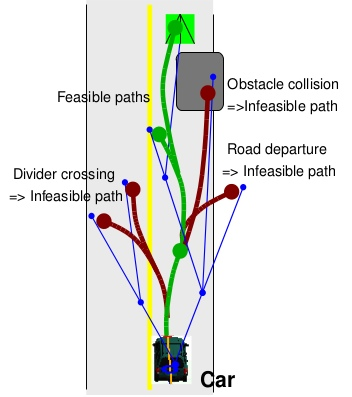
\includegraphics[width=0.5\textwidth]{images/darpa_mit_rrt}
    \caption{Планирование движения с помощью RRT и регулятора с обратной связью}
    \label{img:darpa_mit_rrt}
\end{figure}


Существует Open-Source библиотека The Open Motion Planning Library \cite{motion_planning_ompl}, которая реализует
sample-based алгоритмы поиска, таких как RRT, RRT* и ряд других, основанных на них, как для планирования в
пространстве конфигураций, так и для планирования в пространстве состояний (kinodynamic planning). Библиотека легко
интегрируется с любой задачей планирования движения, поскольку не имеет никаких ограничений на тип задачи, способы
представления препятствий, используемые динамические модели. Программисту достаточно определить вышеназванные
функции $NOT\_COLLIDED$, $PROPAGATE$, $STEER$ в соответствии с используемым способом представления препятствий и моделью
робота. Библиотека имеет ряд готовых реализаций для широко распространенных пространств конфигурации, состояний и
управления, таких как $SO(2)$ , $SO(3)$, $SE(2)$, $SE(3)$, но возможно определить и свои.


\subsection{Методы интерполяции кривыми}

Следующей группой методов, применяемых для реализации задачи планирования движения беспилотного
автомобиля, является интерполяция траектории движения с помощью каких-либо кривых или иных лииний.

Эти алгоритмы принимают набор точек (например, данный набор точек пути, описывающих глобальную дорожную карту),
генерируя новый набор данных (более плавный путь) удовлетворяющий требования на непрерывность траектории,
ограничения транспортного средства и учитывая динамическую среду, в которой движется автомобиль.

В отличие от методов, рассмотренных ранее, которые являются универсальными и могут применяться к решению
различных задач планирования движения, применительно к беспилотному автомобилю, это задача движения
в неструктурированном окружении,  эти методы широко применяются для построения траектории при движении
по дороге.

Планировщики интерполяционных кривых реализуют различные методы сглаживания траектории и генерации кривых.
Могут применяться различные кривые для интерполяции, такие как линии и окружности, клотоиды, кривые Безье
или полиномы. Полиномы зачастую применяются для того, чтобы построить участок траектории, удовлетворяющий
граничным условиям (например, положению и скорости).

Так в работах \cite{darpa_junior_path_planning_1}, \cite{darpa_junior_frenet},
опубликованных по результатам участия команды Стэндфордского университета в Darpa Ubran Challenge,
рассматривается планирование траектории с помощью полиномов пятого порядка в подвижной системе координат,
связанной с желаемой траекторией, основанной на трехграннике Френе.  В этой работе осуществляется независимое
формирование продольной и поперечных траекторий, обе представлены в форме полиномов пятого порядка. Алгоритм генерирует
набор кривых путем варьирования конечных условий, а затем осуществляется выбор оптимальной траектории с использованием
различных функций стоимости.

Стоит отметить, что формирование большого набора траекторий с последующим выбором оптимальной является распространенным
подходов в решении задачи планирования движения.

В работе \cite{motion_planning_interpolate_path_optimization} представлен похожий подход, отличающийся тем, что после
нахождения оптимальной траектории из набора дискретных траекторий, осуществляется дополнительная процедура оптимизации
параметров полиномов с целью получить более оптимальную траекторию.

В работе \cite{motion_planning_interpolate_bezier} применяются кривые Безье пятого порядка для формиирования траектории
движения автомобиля с моделью Аккермана. Алгоритм получает на вход набор путевых точек и формирует путь, проходящий
через них с помощью набора кривых Безье. Каждый сегмент определяется положением точки, первой и второй производной, т.е.
скоростью и ускорением автомобиля. Полученная кривая имеет гладкие стыки между сегментами. Затем осуществляется
оптимизация кривой путем изменения положений и первых производных в опорных точках, чтобы оптимизировать длину пути.

\section{Обзор некоторых систем управления беспилотными автомобилями}

В этом разделе будут более детально рассмотренны некоторые решения в области планирования движения беспилотных автомобилей,
в основном, на основе публикаций участников Darpa Urban Challenge.

\subsection{Команда Junior в Darpa Urban Challenge}

В работах \cite{darpa_junior_path_planning_1}, \cite{darpa_junior_frenet},
опубликованных по результатам участия команды Стэндфордского университета в Darpa Ubran Challenge,
рассматривается планирование траектории с помощью полиномов пятого порядка в подвижной системе координат,
связанной с желаемой траекторией, основанной на трехграннике Френе. Иллюстрация этого способа представлена на
рисунке \ref{img:junior_frenet_frame}, где
$s(t)$  ~--- длина дуги, пройденная автомобилем, $\vec{t}_r$ - направляющий вектор системы координат,
$\vec{n}_r$  ~--- нормальный вектор системы координат, $\vec{x}(s,d)$, $\vec{n}_x$,
$\vec{t}_x$ ~--- положение и направляющие векторы локальной системы координат автомобиля соответственно и
$d(t)$ ~--- отклонение автомобиля от желаемой траектории.

\begin{figure}[h]
    \centering
    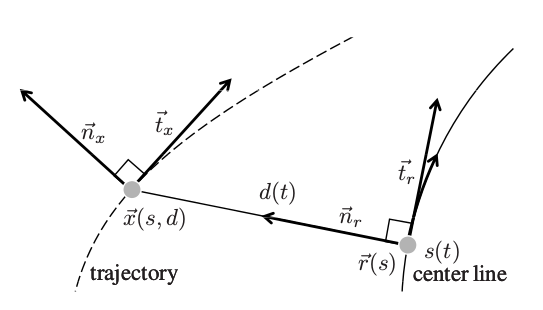
\includegraphics[]{images/junior_frenet_frame}
    \caption{Система координат для планирование траектории}
    \label{img:junior_frenet_frame}
\end{figure}


Планирование осуществляется независимо для продольного и поперечного движения,
а затем полученные полиномы объединяются в траекторию и переводятся в декартову систему координат.
Выбирается оптимальная траектория, минимизирующая функцию стоимости. За основу функции стоимости взят
интеграл третьей производной, рывка (jerk):

\begin{equation}
    J= \int_{t_0}^{t_1}{\dddot{p}^2 d\tau}
\end{equation}

\noindent\begin{tabularx}{\linewidth}{lllX}
    где & $p$         &~---& положение (продольное или поперечное), \\
        & $t_0, t_1$  &~---& время совершения маневра.
\end{tabularx}

Полиномы пятого порядка выбраны по причине того, что оптимальным решением для минимизации этого
интеграла.

Так как при планировании движения требуется учитывать препятствия, задача оптимизации для
нахождения коэффициентов полинома, минимизирующего стоимость крайне затруднительно. Вместо этого
в работе предложен другой подход, являющийся типичным для подомных методов. Формируется набор
траекторий путем варьирования конечных условий, а затем из них выбирается траектория, которая
лучше всего минимизирует функцию стоимости и, при этом, удовлетворяет ограничениям, например:

\begin{eqnarray}
    D_0 = [d_0, \dot{d_0}, \ddot{d_1}] \\
    D_{1_{ij}} = [d_i, 0, 0, T_j]
\end{eqnarray}

\noindent\begin{tabularx}{\linewidth}{lllX}
    где & $D_0, D_1$                    &~---& начальное и конечное состояние, \\
        & $d_0, \dot{d_0}, \ddot{d_0}$  &~---& текущие поперечные положение, скорость и ускорение автомобиля,\\
        & $d_i$                         &~---& конечное поперечное положение,\\
        & $T_j$                         &~---& время выполнения маневра.
\end{tabularx}

Пример планирования поперечных и продольных траекторий представлены на рисунке \ref{img:junior_pathes_lat} и
\ref{img:junior_pathes_lon} соответственно.

\begin{figure}[h]
    \centering
    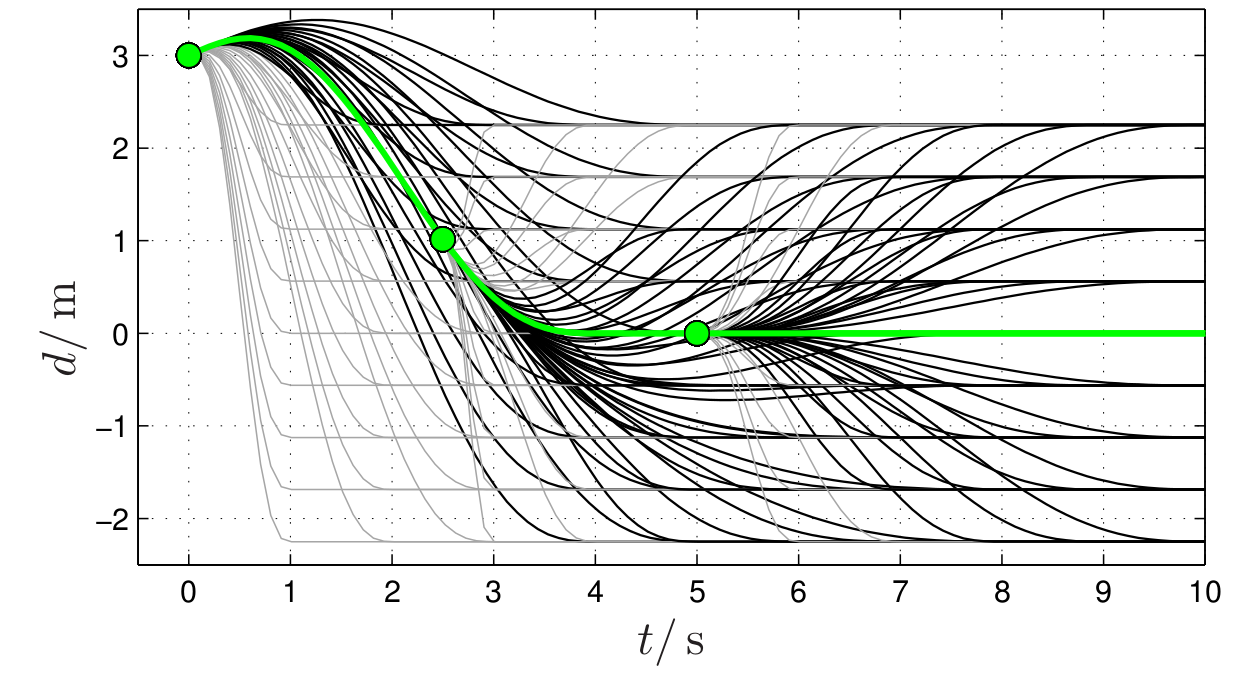
\includegraphics[width=0.7\linewidth]{images/junior_pathes_lat}
    \caption{Планирование поперечного движения, зеленая ~--- оптимальная траектория, черная ~--- валидные траектории,
        серые ~--- невалидные траектории}
    \label{img:junior_pathes_lat}
\end{figure}

\begin{figure}[h]
    \centering
    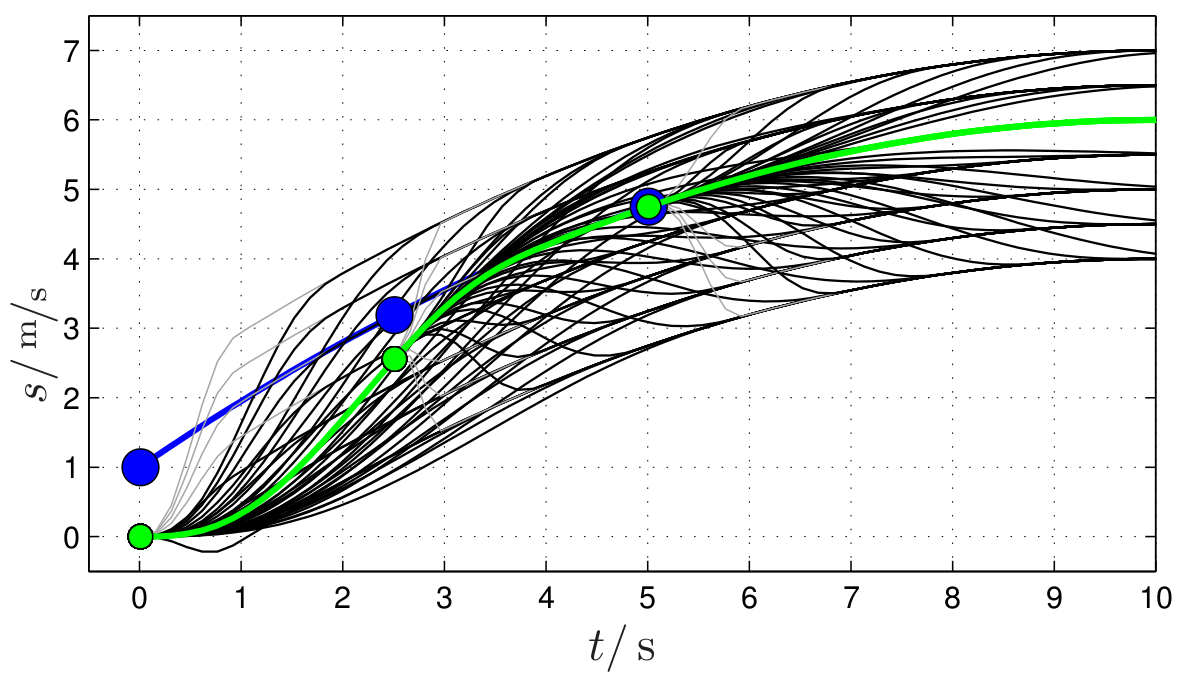
\includegraphics[width=0.7\linewidth]{images/junior_pathes_lon}
    \caption{Планирование продольного движения}
    \label{img:junior_pathes_lon}
\end{figure}

\subsection{Команда BOSS в Darpa Urban Challenge}
Команда BOSS университета  Карнеги-Меллона использовала \cite{darpa_boss}, \cite{darpa_boss_2}, \cite{darpa_boss_3}
несколько иной подход, основанный на методе решеток состояния (state lattice). Планировщик траектории формирует набор
траекторий-кандидатов, из которых затем выбтирается лучшая, удовлетворяющая ограничениям и функции стоимости.

Каждая траектория-кандидат расчитывается с помощью MPC (Model Predictive Control) генератора \cite{darpa_boss_kelly},
который формирует динамически достижимый путь между начальным и конечным состояниями. Этот алгоритм может быть
использован для формирования набора параметризованных последовательностей управления $[u(p,x)]$, которые удовлетворяют
набору ограничений в виде дифференциальных уравнениф вида:
\begin{equation}
\dot{x}(x, p) = f(x, u(p,x))
\end{equation}
где $x$ - состояние автомобиля
(положение $x$, $y$, оринетация $\theta$, кривизна траектории $k$, скорость $v$), $p$ - набор параметров.

Авторы вводят набор ограничений, которые описываются как разница между целевым состоянием $X_c$ и конечной точкой траектории,
получаемой путем интегрирования уравнений динамики автомобиля:
\begin{equation}
    x_c = <x_c, y_c, \theta_c>^T
\end{equation}
\begin{equation}
    x_f(p,x) = x_{i} + \int_0^{t_1}{\dot{x}(x, p)dt}
\end{equation}
\begin{equation}
    C(x, p) = x_c - x_f(p,x)
\end{equation}

Путем минимизации ошибки $C(x, p)$ находятся такие коэффициенты $p$, что полученная траектория как можно ближе подходит
к заданному конечному состоянию.

Траектории определяются функцией скорости $v(p, t)$ и функцией кривизны $k(p, s)$, где $s$ - покрытая длина дуги. В работе
применен ряд различных функций, реализующих различные профили скорости, принимяемые в разных ситуациях
(рисунок \ref{img:boss_velocity_prifiles}а). Функция кривизны опредеяется в виде сплайна второго порядка и задается
набором трех опорных точек (рисунок \ref{img:boss_velocity_prifiles}b). Каждая траектория определяется набором
параметров, которые подбираются в процессе оптимизации.

Траектории расчитываются заранее и формируют lookup-таблицу, с помощью которой определяются подходящие параметры траектории
для состояния, близкого к текущему состоянию автомобиля. Это существенно ускоряет операцию планирования движения.

\begin{figure}[h]
    \centering
    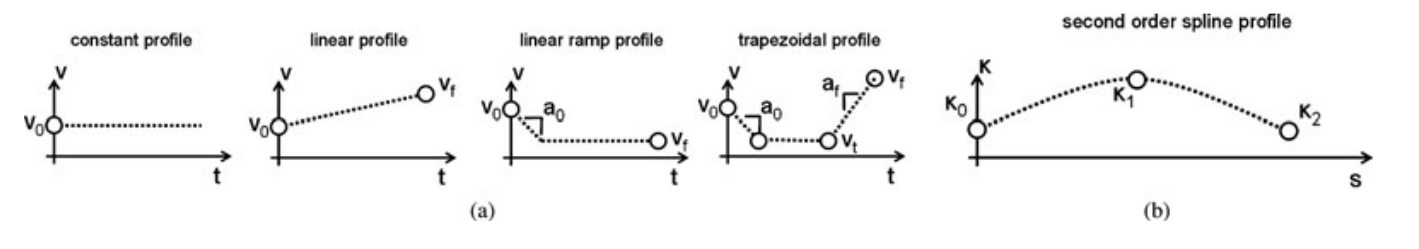
\includegraphics[width=\linewidth]{images/boss_velocity_prifiles}
    \caption{Профили скорости автомобиля BOSS}
    \label{img:boss_velocity_prifiles}
\end{figure}


\begin{figure}[h]
    \centering
    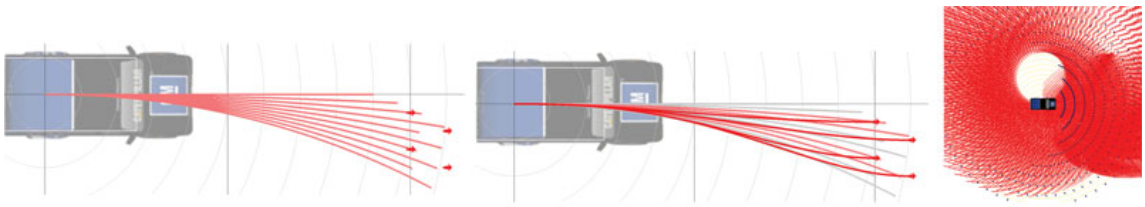
\includegraphics[width=\linewidth]{images/boss_lattice_gen}
    \caption{Предвариетельно расчитанные траектории автомобиля BOSS}
    \label{img:boss_lattice_gen}
\end{figure}

%\subsection{Команда Talos в Darpa Urban Challenge}
%\subsection{Команда AnnieWAY в Darpa Urban Challenge}

\section{Выводы по главе}
Был проведен обзор основных существующих подходов к построению систем управления беспилотными автомобилями,
выделены общие принципы архитектуры системы управления, определены типичные компоненты, входящие в ее состав.
Были рассмотрены различные методы планирования движения применительно к задаче планирования движения
наземного транспортного средства.